\documentclass[border=10pt]{standalone}

\usepackage{tikz}
\usepackage{tikzsymbols}
\usetikzlibrary{calc,patterns,shapes.geometric}

\def\centerarc[#1](#2)(#3:#4:#5){\draw[#1] ($(#2)+({#5*cos(#3)},{#5*sin(#3)})$) arc (#3:#4:#5);}

\begin{document}
	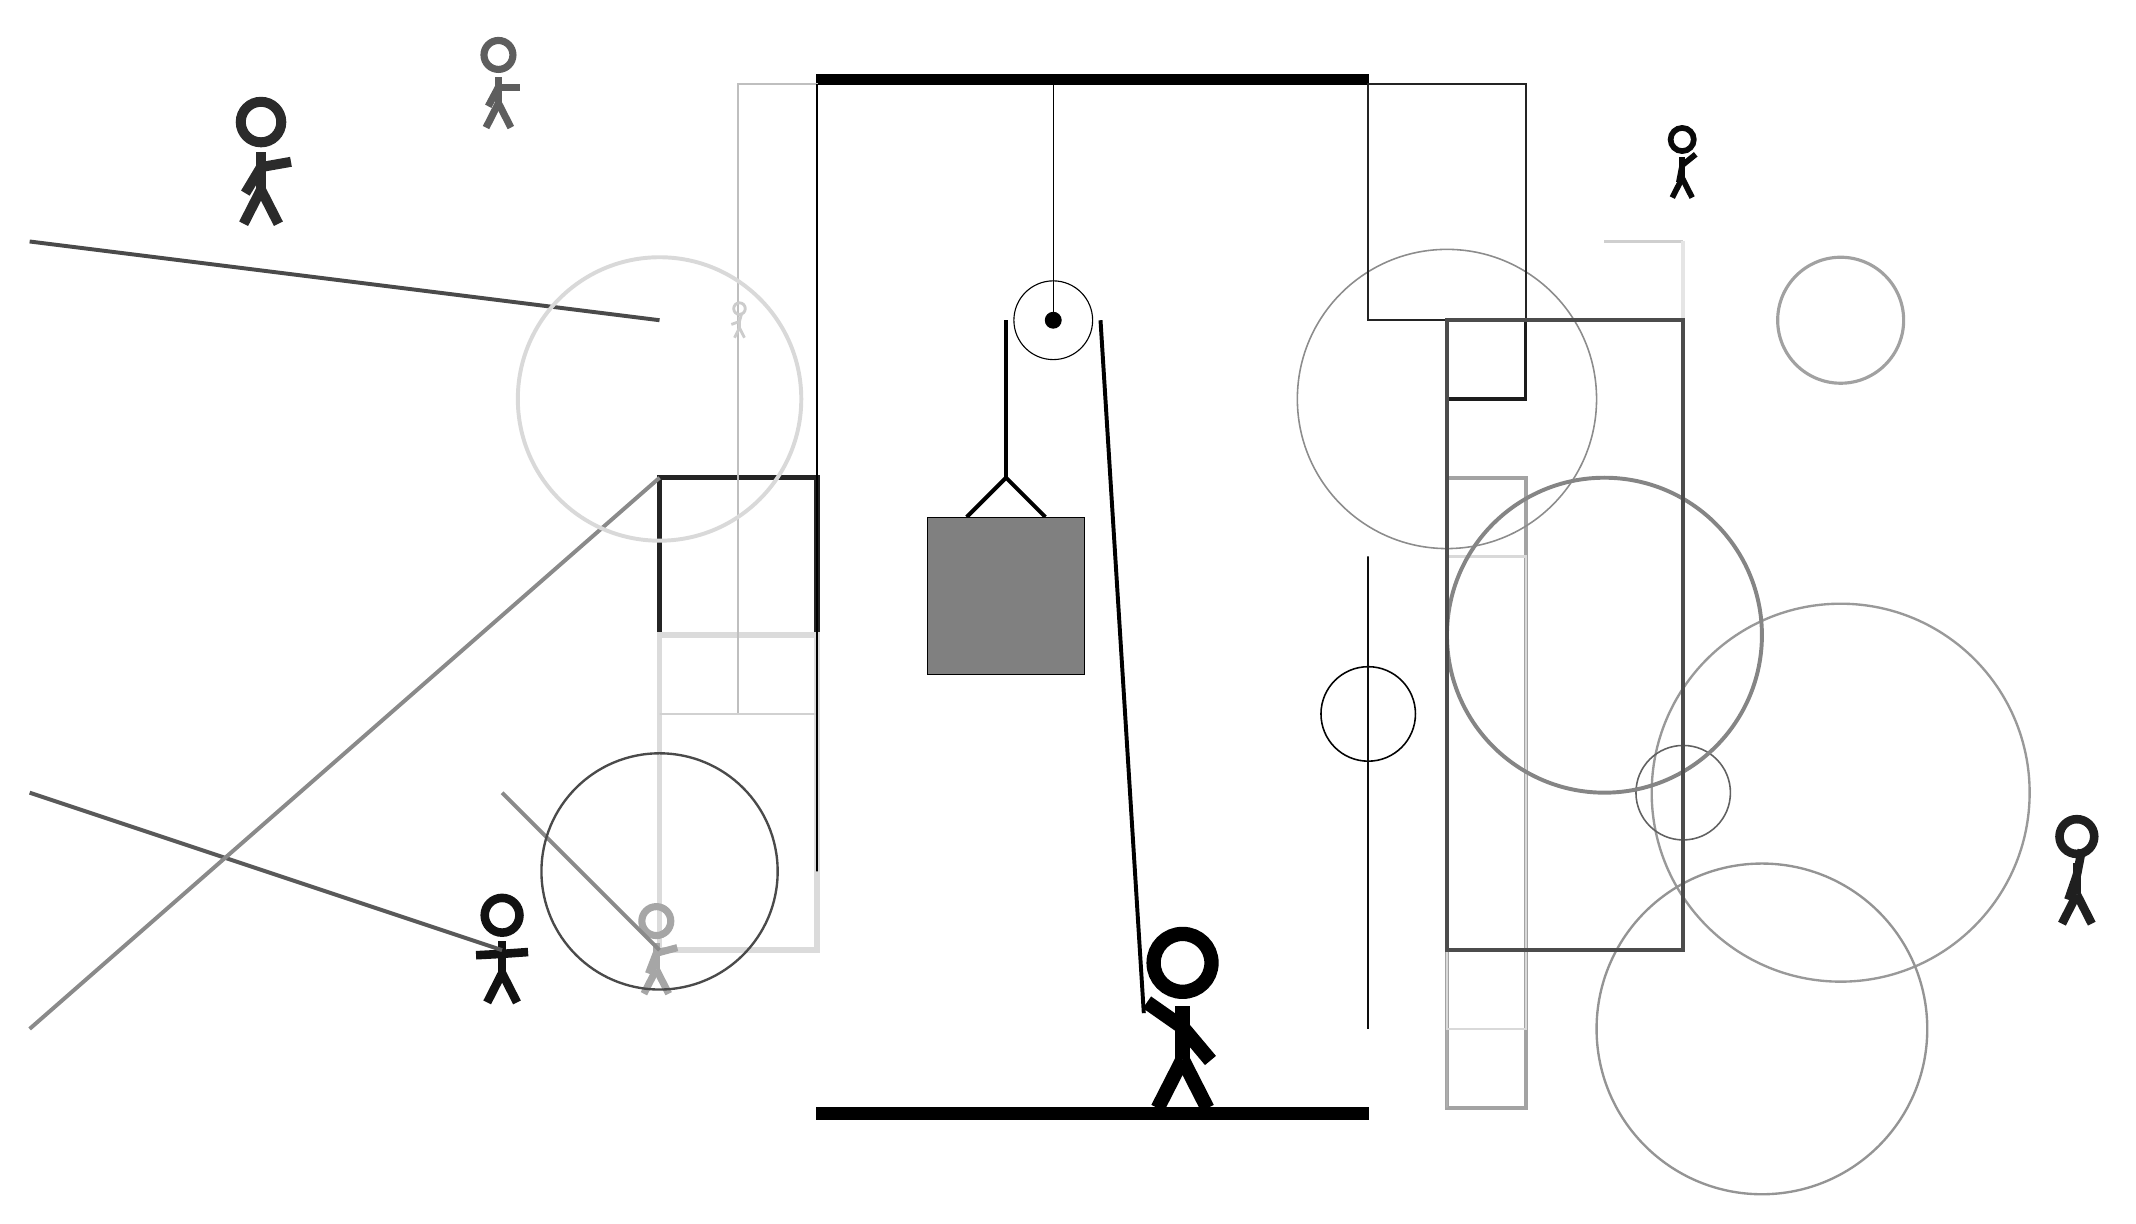
\begin{tikzpicture}
		%%%%% START %%%%%
		
		\draw[fill=black] (-2, 10) rectangle (5, 10.125);
		
		\draw (1, 7) circle (0.5);
		\draw[fill=black] (1, 7) circle (0.1);
		\draw (1, 10) -- (1, 7);
		
		\draw[line width=0.5mm] (-0.1, 4.5) -- (0.4, 5.0) -- (0.9, 4.5);
		\draw[fill=black!50] (-0.6, 4.5) rectangle (1.4, 2.5);
		
		\node[line width=0.3mm, color=black!83] at (-9, 9) {\Strichmaxerl[7][59][10]};
		
		\draw[line width=0.7mm, color=black!86] (-4, -1) rectangle (-2, 5);
		\draw [line width=0.3mm, color=black!40](11, 1) circle (2.4);
		\draw[line width=0.7mm, color=black!14] (-2, 3) rectangle (-4, -1);
		\draw[line width=0.4mm, color=black!89] (7, 7) rectangle (6, 6);
		\draw[line width=0.3mm, color=black!25] (-2, 10) rectangle (-3, 2);
		\node[line width=0.6mm, color=black!35] at (-4, -1) {\Strichmaxerl[5][69][15]};
		\draw[line width=0.5mm, color=black!19](9, 8) -- (8, 8);
		\draw [line width=0.2mm, color=black!99](5, 2) circle (0.6);
		\draw[line width=0.5mm, color=black!71](-4, 7) -- (-12, 8);
		
		\node[line width=0.2mm, color=black!93] at (-6, -1) {\Strichmaxerl[6][3][4]};
		\node[line width=0.2mm, color=black!88] at (14, 0) {\Strichmaxerl[6][71][79]};
		\draw [line width=0.2mm, color=black!62](9, 1) circle (0.6);
		
		\draw[line width=0.5mm, color=black!20](-7, 7) -- (-7, 7);
		\node[line width=0.5mm, color=black!63] at (-6, 10) {\Strichmaxerl[5][62][0]};
		\draw[line width=0.5mm, color=black!36] (7, -3) rectangle (6, 5);
		
		\node[line width=0.2mm, color=black!96] at (9, 9) {\Strichmaxerl[4][79][39]};
		\draw [line width=0.4mm, color=black!37](11, 7) circle (0.8);
		\draw[line width=0.2mm, color=black!32] (6, 3) rectangle (6, -3);
		\draw[line width=0.5mm, color=black!46](-6, 1) -- (-4, -1);
		\draw [line width=0.2mm, color=black!45](6, 6) circle (1.9);
		
		\draw[line width=0.2mm, color=black!86] (7, 10) rectangle (5, 7);
		\draw[line width=0.5mm, color=black!10](9, 8) -- (9, 2);
		\node[line width=0.7mm, color=black!20] at (-3, 7) {\Strichmaxerl[2][20][75]};
		\draw[line width=0.5mm, color=black!65](-6, -1) -- (-12, 1);
		
		\draw[line width=0.5mm, color=black!32] (-3, 0) rectangle (-3, 0);
		\draw[line width=0.3mm, color=black!15] (7, -2) rectangle (6, 4);
		\draw[line width=0.3mm, color=black!18] (-4, 2) rectangle (-2, 2);
		
		\draw[line width=0.3mm, color=black!100] (-2, 10) rectangle (-2, 0);
		\draw [line width=0.3mm, color=black!71](-4, 0) circle (1.5);
		\draw[line width=0.2mm, color=black!95] (5, -2) rectangle (5, 4);
		\draw [line width=0.3mm, color=black!42](10, -2) circle (2.1);
		\draw[line width=0.5mm, color=black!46](-4, 5) -- (-12, -2);
		\draw [line width=0.5mm, color=black!48](8, 3) circle (2.0);
		\draw[line width=0.5mm, color=black!70] (6, 7) rectangle (9, -1);
		\draw [line width=0.5mm, color=black!15](-4, 6) circle (1.8);
		
		\draw[line width=0.5mm] (0.4, 7) -- (0.4, 5.0);
		\centerarc[line width=0.5mm](1, 7)(0:180:0.6);
		\draw[line width=0.5mm](1.6, 7) -- (2.15, -1.8);
		
		\node at (2.6, -1.9) {\Strichmaxerl[10][-35][-50]};
		
		\draw[fill=black] (-2, -3) rectangle (5, -3.15);
		
		%%%%% END %%%%%
	\end{tikzpicture}
\end{document}